\section{Wildcards}
\begin{itemize}
    \item Ways of grabbing data that matches a specific pattern.
    \item Find any client's who are an LLC:
        \begin{minted}[autogobble]{sql}
            SELECT * FROM client WHERE client_name LIKE '%LLC';
        \end{minted}
        \begin{figure}[H]
            \centering
            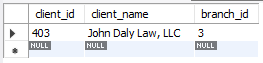
\includegraphics[width=0.4\textwidth]{./Figs/2020-12-24-21-00-45.png}
        % 	\caption{}
        \end{figure}
        \begin{itemize}
            \item The condition will be true if the last three characters of the client name are LLC, the \% wildcard allows you to not specify from which character index you must start.
        \end{itemize}
    
    \item Use characters to define a 'template' for pattern matching.
        \begin{itemize}
            \item \% means any number of characters.
            \item \_ means one character.
        \end{itemize}
    
    \item Find any branch suppliers who are in the label business:
        \begin{minted}[autogobble]{sql}
            SELECT * FROM branch_supplier WHERE supplier_name LIKE '% Label%';
        \end{minted}
        \begin{figure}[H]
            \centering
            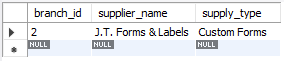
\includegraphics[width=0.4\textwidth]{./Figs/2020-12-24-21-01-12.png}
        % 	\caption{}
        \end{figure}
    
    \item Find any employee born in october:
        \begin{minted}[autogobble]{sql}
            SELECT * FROM employee WHERE birth_day LIKE '____-10%';
        \end{minted}
        \begin{figure}[H]
            \centering
            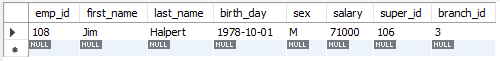
\includegraphics[width=0.4\textwidth]{./Figs/2020-12-24-21-01-33.png}
        % 	\caption{}
        \end{figure}
    
    \item Find any clients who are schools:
        \begin{minted}[autogobble]{sql}
            SELECT * FROM client WHERE client_name LIKE '%school%';
        \end{minted}
        \begin{figure}[H]
            \centering
            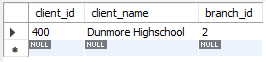
\includegraphics[width=0.4\textwidth]{./Figs/2020-12-24-21-01-53.png}
        % 	\caption{}
        \end{figure}
\end{itemize}
